\documentclass[varwidth=true, border=2pt]{standalone}

\usepackage{pgfplots}
\usepackage{tikz}

\usetikzlibrary{calc,patterns,angles,quotes}

\begin{document}

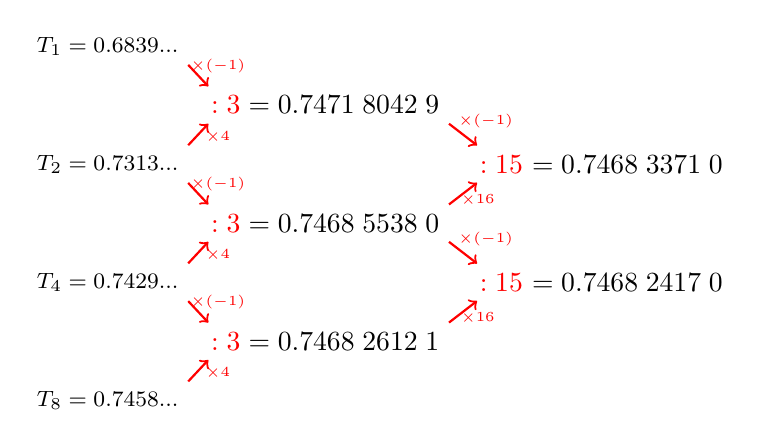
\begin{tikzpicture}


	\node (T1) at (1,5.25) {\footnotesize{$T_1 = 0.6839...$}};
	\node (T2) at (1,3.75) {\footnotesize{$T_2 = 0.7313...$}};
	\node (T4) at (1,2.25) {\footnotesize{$T_4 = 0.7429...$}};
	\node (T8) at (1,.75) {\footnotesize{$T_8 = 0.7458...$}}; %Some uncertainty about last 2 digits.  Maybe recalculate in MATLAB
	\node (A1)[red] at (2.5, 4.5){$:3$};
	\node (A2)[red] at (2.5, 3){$:3$};
	\node (A3)[red] at (2.5, 1.5){$:3$};
	
	\node (B1)at (4,4.5){$= 0.7471\;8042\;9$};
	\node (B2) at (4,3){$= 0.7468\;5538\;0$};
	\node (B3) at (4,1.5){$= 0.7468\;2612\;1$};
	\node (D1)[red] at (6, 3.75){$:15$};
	\node (D2)[red] at (6, 2.25){$:15$};
	
	\node (E1) at (7.6,3.75){$= 0.7468\;3371\;0$};
	\node (E1) at (7.6,2.25){$= 0.7468\;2417\;0$};
	
%	\node (F1)[red] at (11, 4){$:63$};

	\draw [->, thick,red] (T1.south east) to (A1);
	\draw [->, thick,red] (T2.north east) to (A1);
	\draw [->, thick,red] (T2.south east) to (A2);
	\draw [->, thick,red] (T4.north east) to (A2);
	\draw [->, thick,red] (T4.south east) to (A3);
	\draw [->, thick,red] (T8.north east) to (A3);

	\draw [->, thick,red] (B1.south east) to (D1);
	\draw [->, thick,red] (B2.north east) to (D1);
	\draw [->, thick,red] (B2.south east) to (D2);
	\draw [->, thick,red] (B3.north east) to (D2);

	\node (A1a)[red] at (2.4,5){\tiny{$\times (-1)$}};
	\node (A1b)[red] at (2.4,4.1){\tiny{$\times 4$}};
	\node (A2a)[red] at (2.4,3.5){\tiny{$\times (-1)$}};	
	\node (A2b)[red] at (2.4,2.6){\tiny{$\times 4$}};
	\node (A3a)[red] at (2.4,2){\tiny{$\times (-1)$}};	
	\node (A3b)[red] at (2.4,1.1){\tiny{$\times 4$}};

	\node (D1a)[red] at (5.8,4.3){\tiny{$\times (-1)$}};
	\node (D1b)[red] at (5.7,3.3){\tiny{$\times 16$}};
	\node (D2a)[red] at (5.8,2.8){\tiny{$\times (-1)$}};
	\node (D2b)[red] at (5.7,1.8){\tiny{$\times 16$}};	
	
\normalsize
	
\end{tikzpicture}
\end{document}